\documentclass{article}
\usepackage[a4paper]{geometry}
\usepackage{fancyhdr}
\usepackage{hyperref} 
\usepackage{tikz}
\usepackage{amsmath} 
\pagestyle{fancy}
\lhead{Winkel}
\rhead{Juli 2025}
\begin{document}
   
\newcommand{\norm}[1]{\big| {#1} \big|}  
\newcommand{\vect}[1]{\overrightarrow{#1}} 
 
\section{Winkel}
\subsection{Zwischen zwei Vektoren} 
\begin{minipage}[t]{\dimexpr\textwidth-4cm} 
Sind zwei Vektoren, $\vect{a}$ und $\vect{b}$, mit einem Winkel $\alpha$ gegeben, ist es offensichtlich, dass
\[
 \vect{a} = \begin{pmatrix} \norm{\vect{a}} \\ 0 \end{pmatrix}
 \quad \text{und} \quad 
 \vect{b} = \begin{pmatrix} \cos(\alpha) \norm{\vect{b}} \\ \sin(\alpha) \norm{\vect{b}} \end{pmatrix}
\]
Demnach folgt
\end{minipage} 
\hfill
\begin{minipage}[t]{4cm} 
 \centering 
 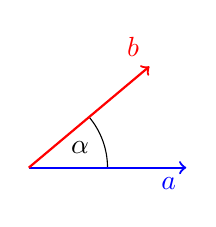
\begin{tikzpicture}[baseline=(current bounding box.north)]
  \coordinate (mid) at (0,0); 
  \path (mid) ++(2, 0) coordinate (enda);
  \path (mid) ++({2*sin(50)}, {2*cos(50)}) coordinate (endb);
 
  \draw (mid) ++(1, 0) arc[start angle=0, end angle=40, radius=1]; 
  \draw (mid) ++(0.65, 0.25) node {$\alpha$}; 
 
  \draw[->, thick,blue] (mid) -- (enda) node [below left] {$\vect{a}$};
  \draw[->, thick,red] (mid) -- (endb) node [above left] {$\vect{b}$};
 \end{tikzpicture} 
\end{minipage}
\begin{align*}
 \vect{a} \cdot \vect{b} &= \norm{\vect{a}} \cdot \cos(\alpha) \norm{\vect{b}} - \sin(\alpha) \norm{\vect{b}} \cdot 0 \\
 &= \norm{\vect{a}} \cdot \norm{\vect{b}} \cdot \cos(\alpha) \\
 \cos(\alpha) &= \frac{\vect{a} \cdot \vect{b}}{\norm{\vect{a}} \cdot  
\norm{\vect{b}}} \\ 
 \alpha &= \cos^{-1}\left({\frac{\vect{a} \cdot \vect{b}}{\norm{\vect{a}} \cdot  \norm{\vect{b}}}}\right)
\end{align*}
Dies gilt, wie andersweitig ausführlicher Bewiesen werden kann, für alle zwei Vektoren.
 Beim eingeben im Taschenrechner muss hier extra genau auf die Eingabe geachtet werden, weil, insbesondere hier, diejenigen Operationen, welche eigentlich gleich notiert werden, im Taschenrechner andere Funktionen benötigen. Mehr dazu im Kapitel \hyperref[Umgang mit dem Taschenrecher]{Umgang mit dem Taschenrecher}. Somit gilt im Taschenrechner
\[ 
 \alpha =
 \texttt{cos}^{-\texttt{1}}\left(
 \frac{\texttt{dotP(a,b)}}{\texttt{norm(a)}\cdot\texttt{norm(b)}}
 \right) 
\] 
  
\subsection{Zwischen zwei Geraden} 
\begin{minipage}[t]{4cm}
 \centering 
 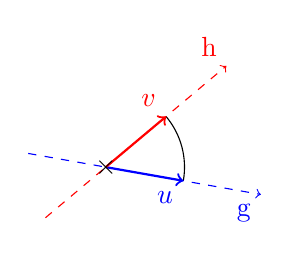
\begin{tikzpicture}[baseline=(current bounding box.north)]
  \coordinate (mid) at (0,0); 
  \path (mid) ++({-1*sin(100)}, {-1*cos(100)}) coordinate (startg);
  \path (mid) ++({2*sin(100)}, {2*cos(100)}) coordinate (endg);
  \path (mid) ++({-1*sin(50)}, {-1*cos(50)}) coordinate (starth);
  \path (mid) ++({2*sin(50)}, {2*cos(50)}) coordinate (endh);
  \path (mid) ++({1*sin(100)}, {1*cos(100)}) coordinate (endu);  
  \path (mid) ++({1*sin(50)}, {1*cos(50)}) coordinate (endv); 
 
  \draw (mid) ++(endu) arc[start angle=-10, end angle=40, radius=1];  
 
  \draw[->,blue,dashed] (startg) -- (endg) node [below left] {$\mathrm{g}$};
  \draw[->,red,dashed] (starth) -- (endh) node [above left] {$\mathrm{h}$};
  \draw[->,thick,blue] (mid) -- (endu) node [below left] {$\vect{u}$};
  \draw[->,thick,red] (mid) -- (endv) node [above left] {$\vect{v}$}; 
  \draw (mid) node {$\times$};  
 \end{tikzpicture} 
\end{minipage} 
\hfill
\begin{minipage}[t]{\dimexpr\textwidth-4cm}
Werden beim Schnittpunkt von zwei Geraden jeweils ihre Richtungsvektoren eingezeichnet, wird offensichtlich, dass der Winkel zwischen den zwei Geraden auch der Winkel zwischen ihren beiden Richtungsvektoren ist. Haben die die beiden Geraden $\mathrm{g}$ und $\mathrm{h}$ die Richtungsvektoren $\vect{u}$ und $\vect{v}$, so ist der Winkel $\alpha$ 
\[
 \alpha = \cos^{-1}\left({\frac{\vect{u} \cdot \vect{v}}{\norm{\vect{u}} \cdot  \norm{\vect{v}}}}\right)
\] 
\end{minipage}
 
\subsection{Zwischen Ebene und Gerade}
\begin{minipage}[t]{\dimexpr\textwidth-5cm} 
% todo: erklärung cos a' = ..., a' = 90-a, cos(a-90) = sin(a)
% HIER und nächste || für spitzen winkel -n 
Weil die Richtungsvektoren in der Regel nicht der Ebene entlang in die gleiche Richtung wie der Richtungsvektor der Gerade zeigen, wird stattdessen der Normalvektor der Ebene genutzt. Dabei wird aber das Skalarprodukt, weil $\vect{n}$ auf der anderen Seite der Ebene sein könnte, so wie es hier $-\vect{n}$ ist, welches zu einem stumpfen Winkel als Ergebniss folgen würde, als betrag genommen. Somit gilt für den Winkel $\alpha'$ zwischen einer Gerade mit dem Richtungsvektor $\vect{u}$ und einer Ebene
\end{minipage} 
\hfill
\begin{minipage}[t]{5cm} 
 \centering 
 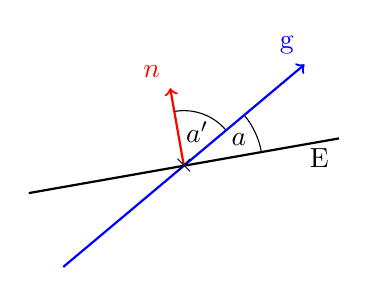
\begin{tikzpicture}[baseline=(current bounding box.north)]
  \coordinate (mid) at (0,0); 
  \path (mid) ++({-2*sin(80)}, {-2*cos(80)}) coordinate (starte);
  \path (mid) ++({2*sin(80)}, {2*cos(80)}) coordinate (ende);
  \path (mid) ++({-2*sin(50)}, {-2*cos(50)}) coordinate (startg);
  \path (mid) ++({2*sin(50)}, {2*cos(50)}) coordinate (endg);
  \path (mid) ++({1*sin(-10)}, {1*cos(-10)}) coordinate (endn);
  
  \path (mid) ++({1*sin(50)}, {1*cos(50)}) coordinate (posgangle);
  \path (mid) ++({0.7*sin(-10)}, {0.7*cos(-10)}) coordinate (posnangle);
 
  \draw (posnangle) arc[start angle=100, end angle=40, radius=0.7]; 
  \draw (posgangle) arc[start angle=40, end angle=10, radius=1];
 
  \draw[thick,black] (starte) -- (ende) node [below left] {$\mathrm{E}$};
  \draw[->, thick,blue] (startg) -- (endg) node [above left] {$\mathrm{g}$};
  \draw[->, thick,red] (mid) -- (endn) node [above left] {$\vect{n}$}; 
   
  \draw (mid) ++ (0.17, 0.43) node {$a^\prime$};  
  \draw (mid) ++ (0.7, 0.33) node {$a$};  
 
  \draw (mid) node {$\times$}; 
 \end{tikzpicture} 
\end{minipage}
 
\vspace{0.9em}
\[
 \alpha' = \cos^{-1}\left({\frac{\norm{\vect{u} \cdot \vect{n}}}{\norm{\vect{u}} \cdot  \norm{\vect{n}}}}\right)
\] 
Weil $\alpha$, nicht $\alpha'$, gesucht wird, ist anzumerken, dass immer ${\alpha + \alpha' = 90 \Leftrightarrow \alpha' = 90-\alpha}$, sodass $90-\alpha=\cos^{-1}(...)$, weshalb $\cos{(90-\alpha)}=...$ und $\cos{(90-\alpha)}=\sin{(\alpha)}$. Somit gilt
\[
 \alpha = \sin^{-1}\left({\frac{\norm{\vect{u} \cdot \vect{n}}}{\norm{\vect{u}} \cdot  \norm{\vect{n}}}}\right)
\]
Im Taschenrechner gilt
\[ 
 \alpha =
 \texttt{sin}^{-\texttt{1}}\left(
 \frac{\texttt{abs(dotP(u,n))}}{\texttt{norm(u)}\cdot\texttt{norm(n)}}
 \right) 
\] 
  
\subsection{Zwischen zwei Ebenen} 
\begin{minipage}[t]{5cm} 
 \centering 
 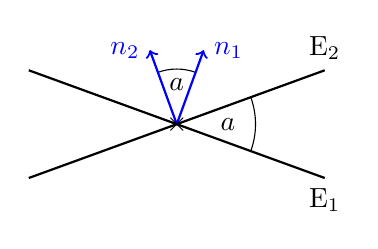
\begin{tikzpicture}[baseline=(current bounding box.north)]
  \coordinate (mid) at (0,0); 
  \path (mid) ++({-2*sin(110)}, {-2*cos(110)}) coordinate (starte1);
  \path (mid) ++({2*sin(110)}, {2*cos(110)}) coordinate (ende1);
  \path (mid) ++({1*sin(20)}, {1*cos(20)}) coordinate (endn1);
  \path (mid) ++({-2*sin(70)}, {-2*cos(70)}) coordinate (starte2);
  \path (mid) ++({2*sin(70)}, {2*cos(70)}) coordinate (ende2);
  \path (mid) ++({1*sin(-20)}, {1*cos(-20)}) coordinate (endn2);
  
  \path (mid) ++({1*sin(70)}, {1*cos(70)}) coordinate (poseangle);
  \path (mid) ++({0.7*sin(-20)}, {0.7*cos(-20)}) coordinate (posnangle);
  
  \draw (poseangle) arc[start angle=20, end angle=-20, radius=1];
  \draw (posnangle) arc[start angle=110, end angle=70, radius=0.7]; 
 
  \draw[thick,black] (starte1) -- (ende1) node [below] {$\mathrm{E}_1$}; 
  \draw[thick,black] (starte2) -- (ende2) node [above] {$\mathrm{E}_2$};
  \draw[->, thick,blue] (mid) -- (endn1) node [right] {$\vect{n_1}$};
  \draw[->, thick,blue] (mid) -- (endn2) node [left] {$\vect{n_2}$}; 
   
  \draw (mid) ++ (0, 0.5) node {$a$};  
  \draw (mid) ++ (0.65, 0) node {$a$};  
 
  \draw (mid) node {$\times$}; 
 \end{tikzpicture} 
\end{minipage} 
\hfill
\begin{minipage}[t]{\dimexpr\textwidth-5cm}
Mit den obigen Begründungen werden auch beim Berechnen des Winkels zwischen zwei Ebenen die beiden Normalvektoren und Betragsstriche genutzt. Der Winkel zwischen den beiden Normalvektoren ist bereits der Winkel zwischen den beiden Ebenen, somit gilt
\[
 \alpha = \cos^{-1}\left({\frac{\norm{\vect{n_1} \cdot \vect{n_2}}}{\norm{\vect{n_1}} \cdot \norm{\vect{n_2}}}}\right) 
\] 
\end{minipage} 
\end{document} 
 
 
 
